\documentclass{article}
\usepackage[utf8]{inputenc}
\usepackage{amsmath}
\usepackage{graphicx}
\usepackage{tikz}
\usetikzlibrary{patterns}
\title{Homework 3}
\author{Intro to Robotics}
\date{Due Date: May 10th, 2023}

\begin{document}

\maketitle
\section{Quaternions}
1. rotate the 3d vector $P_{1}=\begin{bmatrix}
-1  \\
2 \\
3
\end{bmatrix}$ by $175^{\circ}$ on xz plane and then $35^{\circ}$ on the yz plane using quaternions. \\
2. Convert ${}^{A}_{B}R_{Z'Y'X'}(50^\circ, 150^\circ, 200^\circ)$ to quaternion coordinates.\\
3. Convert rotation matrix $R=\begin{bmatrix}
.28 & .77 & .57\\
-.94 & .34 & 0 \\
-.19 & -.54 & .82
\end{bmatrix}$ to quaternion coordinates.\\
4. consider quaternion $q_{1}$ = (0.845 +0.191i +0.462j +0.191k), convert to $R_{Z'Y'X'}(\alpha,\beta,\gamma)$.
5.  Write a function that rotates 3d vectors using quaternions to verify your answers for 1-3.\\
6. Write a function that takes a rotation matrix as input and returns the equivalent quaternions.\\
7. Write a function that takes a quaternions as input and returns the equivalent rotation matrix.
\newpage
\section{Kinematics 1}
\begin{figure}[htp]
    \centering
    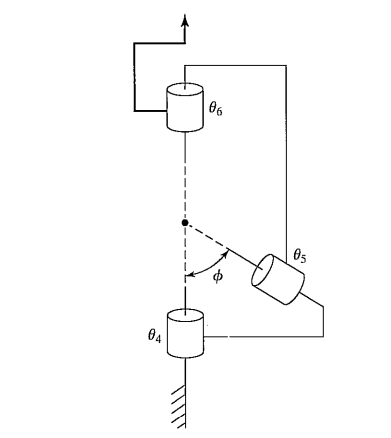
\includegraphics[width=8cm]{arm schematic1.png}
    \caption{}
    \label{fig:Arm}
\end{figure}
1. Compute the frames, dh table and rotation matrices for the given schematic.
\newpage

\section{Kinematics 2}
\begin{figure}[htp]
    \centering
    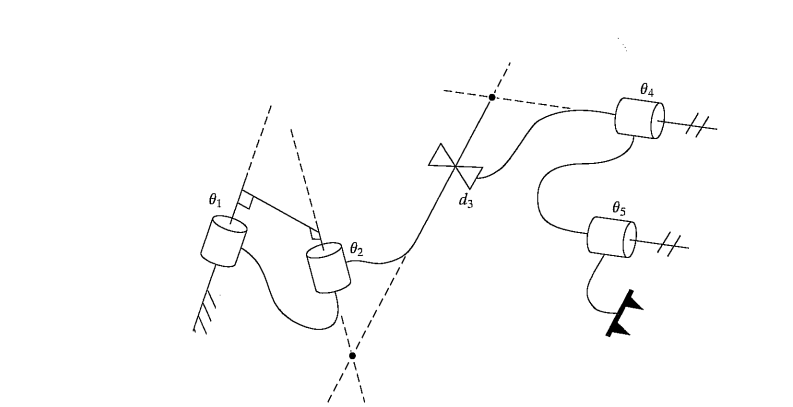
\includegraphics[width=12cm]{arm schematic2.png}
    \caption{}
    \label{fig:Arm}
\end{figure}
1. Compute the frames, dh table and rotation matrices for the given schematic.

\end{document}
